\subsubsection{Module 3: Hoạt động Thương mại}
Đây là phân hệ lõi (Core Domain) của hệ thống Social Commerce, nơi diễn ra các hoạt động trao đổi, mua bán hàng hóa giữa các người dùng.

\begin{figure}[H]
\centering
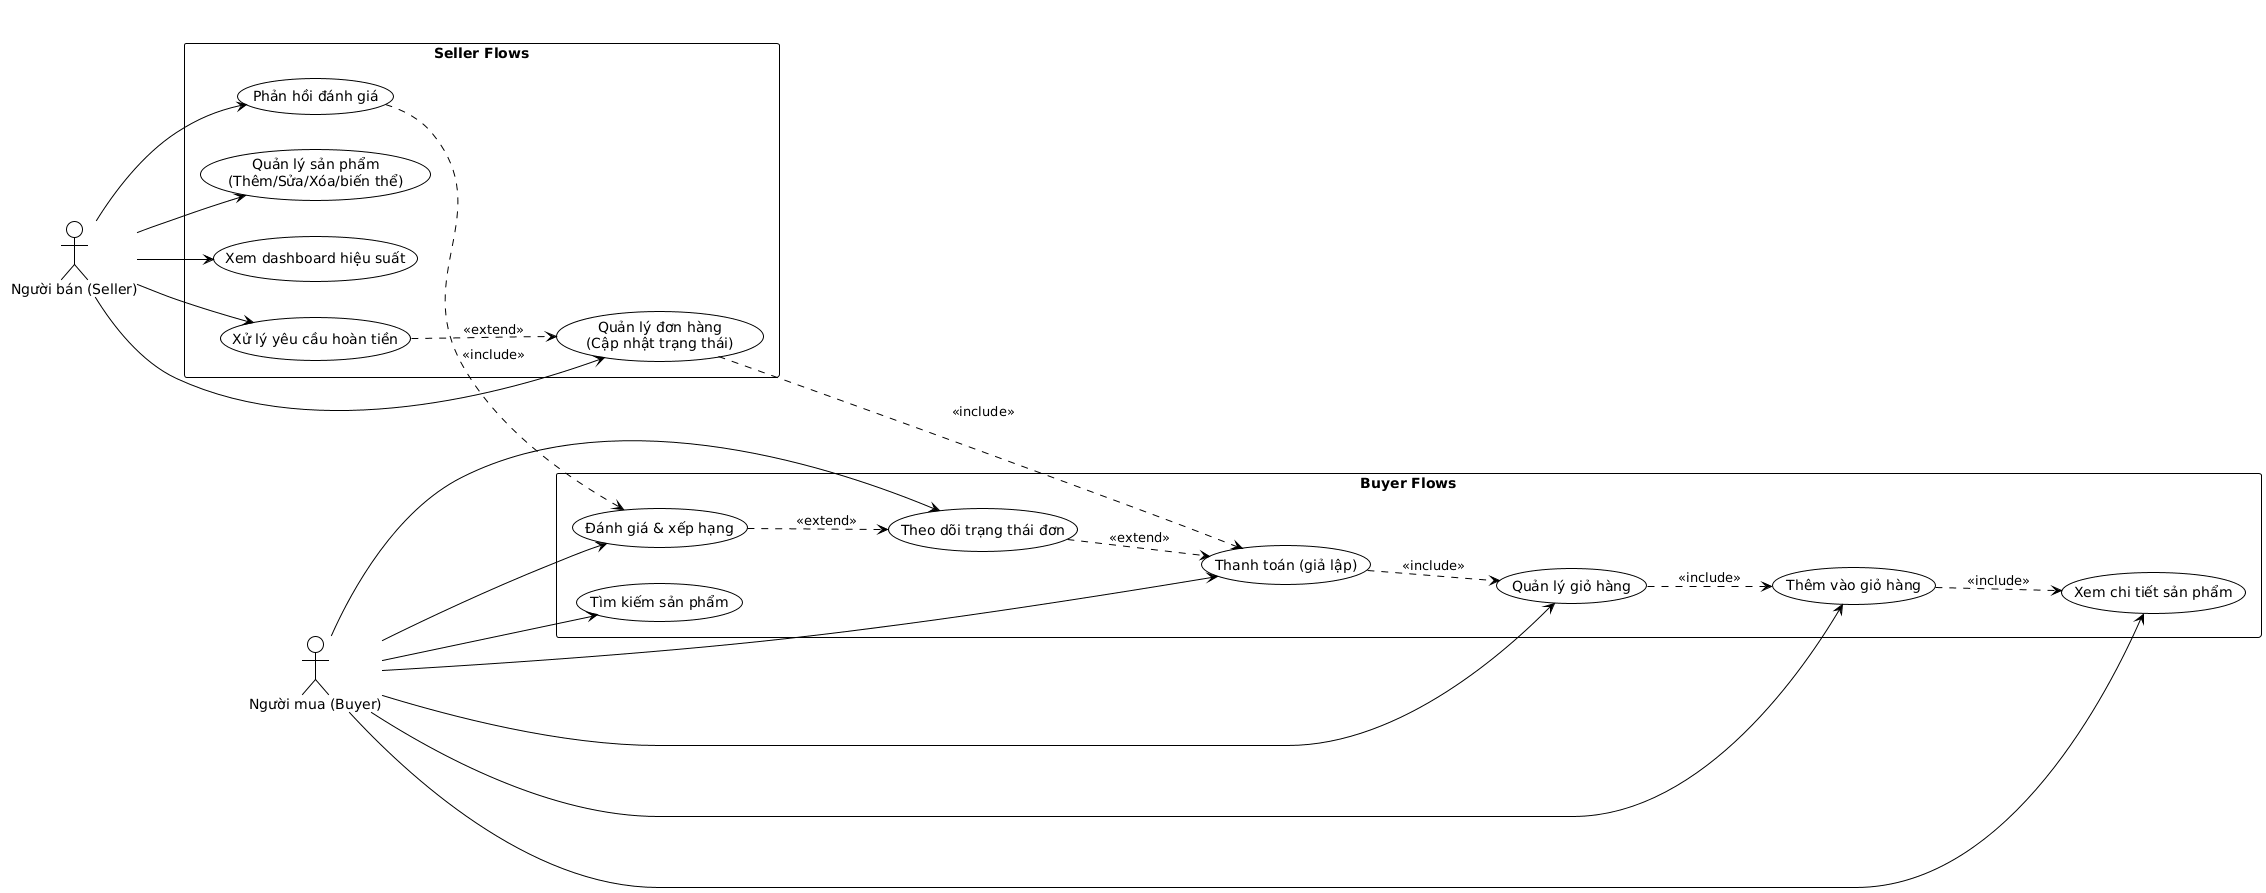
\includegraphics[width=\textwidth]{Images/Usecases/UC-M3-Commerce.png}
\caption{Sơ đồ Use Case cho Module 3: Hoạt động Thương mại}
\label{fig:usecase-module3}
\end{figure}

\renewcommand{\arraystretch}{1.3}

% =====================================================
% PHẦN 1: DÀNH CHO NGƯỜI MUA (BUYER)
% =====================================================
\paragraph{A. Các chức năng dành cho Người mua (Buyer)}

% UC3.1: TÌM KIẾM SẢN PHẨM
\begin{table}[H]
\centering
\begin{tabularx}{\textwidth}{|l|X|}
\hline
\textbf{Tên Use Case} & \textbf{UC3.1: Tìm kiếm sản phẩm} \\ \hline
\textbf{Tác nhân} & Người mua (Buyer) \\ \hline
\textbf{Mô tả} & Cho phép người mua tìm kiếm các sản phẩm họ quan tâm bằng cách sử dụng thanh tìm kiếm và các bộ lọc chi tiết như danh mục và thẻ (tags). \\ \hline
\textbf{Kích hoạt} & Người mua nhập từ khóa vào thanh tìm kiếm hoặc chọn các bộ lọc trên trang sản phẩm. \\ \hline
\textbf{Điều kiện tiên quyết} & Người mua có thể đã đăng nhập hoặc chưa. \\ \hline
\textbf{Điều kiện sau} & Một danh sách các sản phẩm phù hợp với tiêu chí tìm kiếm được hiển thị cho người mua. \\ \hline
\textbf{Luồng sự kiện chính} & 
\begin{enumerate}
    \item Người mua truy cập trang khám phá sản phẩm.
    \item Người mua nhập từ khóa vào thanh tìm kiếm.
    \item Người mua tùy chọn áp dụng các bộ lọc.
    \item Hệ thống truy vấn cơ sở dữ liệu và trả về danh sách sản phẩm khớp.
    \item Giao diện hiển thị kết quả tìm kiếm cho người mua.
\end{enumerate} \\ \hline
\textbf{Ngoại lệ} & E1: Không tìm thấy sản phẩm nào $\rightarrow$ Hệ thống hiển thị thông báo ``Không tìm thấy kết quả phù hợp''. \\ \hline
\end{tabularx}
\caption{Đặc tả Use Case Tìm kiếm sản phẩm}
\end{table}

% UC3.2: XEM CHI TIẾT SẢN PHẨM
\begin{table}[H]
\centering
\begin{tabularx}{\textwidth}{|l|X|}
\hline
\textbf{Tên Use Case} & \textbf{UC3.2: Xem chi tiết sản phẩm} \\ \hline
\textbf{Tác nhân} & Người mua \\ \hline
\textbf{Mô tả} & Cho phép người mua xem thông tin chi tiết về một sản phẩm, bao gồm hình ảnh, mô tả, giá, các biến thể, thông tin người bán và các đánh giá. \\ \hline
\textbf{Kích hoạt} & Người mua nhấp vào một sản phẩm từ kết quả tìm kiếm, Bảng tin hoặc bất kỳ đâu trên nền tảng. \\ \hline
\textbf{Điều kiện tiên quyết} & Sản phẩm phải tồn tại và đang được bán. \\ \hline
\textbf{Điều kiện sau} & Người mua nắm được đầy đủ thông tin về sản phẩm để ra quyết định mua hàng. \\ \hline
\textbf{Luồng sự kiện chính} & 
\begin{enumerate}
    \item Người mua nhấp vào một sản phẩm.
    \item Hệ thống tải và hiển thị trang chi tiết sản phẩm với đầy đủ thông tin.
    \item Người mua có thể xem các hình ảnh, chọn các biến thể (nếu có) và đọc các đánh giá.
\end{enumerate} \\ \hline
\textbf{Ngoại lệ} & E1: Sản phẩm không còn tồn tại hoặc đã bị ẩn $\rightarrow$ Hệ thống hiển thị trang lỗi ``Sản phẩm không tìm thấy''. \\ \hline
\end{tabularx}
\caption{Đặc tả Use Case Xem chi tiết sản phẩm}
\end{table}

% UC3.3: THÊM VÀO GIỎ HÀNG
\begin{table}[H]
\centering
\begin{tabularx}{\textwidth}{|l|X|}
\hline
\textbf{Tên Use Case} & \textbf{UC3.3: Thêm sản phẩm vào giỏ hàng} \\ \hline
\textbf{Tác nhân} & Người mua \\ \hline
\textbf{Mô tả} & Cho phép người mua thêm sản phẩm, bao gồm các biến thể đã chọn, vào giỏ hàng của mình. Người mua có thể thêm sản phẩm từ nhiều cửa hàng khác nhau. \\ \hline
\textbf{Điều kiện tiên quyết} & 
\begin{itemize}
    \item Người mua đã đăng nhập vào hệ thống.
    \item Người mua đã chọn đầy đủ các biến thể bắt buộc của sản phẩm (nếu có).
\end{itemize} \\ \hline
\textbf{Điều kiện sau} & 
\begin{itemize}
    \item Sản phẩm được thêm vào giỏ hàng của người mua.
    \item Biểu tượng giỏ hàng trên giao diện được cập nhật số lượng.
\end{itemize} \\ \hline
\textbf{Luồng sự kiện chính} & 
\begin{enumerate}
    \item Trên trang chi tiết sản phẩm, người mua chọn số lượng và các biến thể mong muốn.
    \item Người mua nhấn ``Thêm vào giỏ hàng''.
    \item Hệ thống xác định biến thể theo \textit{variantId} (hoặc map từ lựa chọn biến thể), kiểm tra trạng thái sản phẩm và tồn kho.
    \item Hệ thống thêm mới hoặc cập nhật cart item tương ứng trong giỏ hàng của người mua.
    \item Hệ thống hiển thị thông báo thành công.
\end{enumerate} \\ \hline
\textbf{Ngoại lệ} & E1: Sản phẩm đã hết hàng $\rightarrow$ Hệ thống báo lỗi và không cho phép thêm vào giỏ. \\ \hline
\end{tabularx}
\caption{Đặc tả Use Case Thêm vào giỏ hàng}
\end{table}

% UC3.4: QUẢN LÝ GIỎ HÀNG
\begin{table}[H]
\centering
\begin{tabularx}{\textwidth}{|l|X|}
\hline
\textbf{Tên Use Case} & \textbf{UC3.4: Quản lý giỏ hàng} \\ \hline
\textbf{Tác nhân} & Người mua \\ \hline
\textbf{Mô tả} & Cho phép người mua xem lại tất cả sản phẩm trong giỏ hàng, cập nhật số lượng, hoặc xóa sản phẩm khỏi giỏ hàng trước khi thanh toán. \\ \hline
\textbf{Kích hoạt} & Người mua nhấp vào biểu tượng giỏ hàng. \\ \hline
\textbf{Điều kiện tiên quyết} & Người mua đã đăng nhập và có ít nhất một sản phẩm trong giỏ hàng. \\ \hline
\textbf{Điều kiện sau} & Giỏ hàng của người mua được cập nhật theo các thay đổi (số lượng, sản phẩm bị xóa). \\ \hline
\textbf{Luồng sự kiện chính} & 
\begin{enumerate}
    \item Người mua truy cập trang giỏ hàng.
    \item Hệ thống hiển thị danh sách các sản phẩm đã thêm.
    \item Người mua có thể: Tăng/giảm số lượng hoặc xóa sản phẩm.
    \item Hệ thống tự động cập nhật lại tổng số tiền.
\end{enumerate} \\ \hline
\textbf{Ngoại lệ} & E1: Cập nhật số lượng vượt quá số lượng tồn kho $\rightarrow$ Hệ thống báo lỗi. \\ \hline
\end{tabularx}
\caption{Đặc tả Use Case Quản lý giỏ hàng}
\end{table}

% UC3.5: THANH TOÁN
\begin{table}[H]
\centering
\begin{tabularx}{\textwidth}{|l|X|}
\hline
\textbf{Tên Use Case} & \textbf{UC3.5: Thực hiện thanh toán} \\ \hline
\textbf{Tác nhân} & Người mua \\ \hline
\textbf{Mô tả} & Cho phép người mua hoàn tất quy trình mua sắm bằng cách cung cấp thông tin giao hàng và thực hiện thanh toán qua một giao diện giả lập. \\ \hline
\textbf{Điều kiện tiên quyết} & 
\begin{itemize}
    \item Người mua đã đăng nhập.
    \item Giỏ hàng có ít nhất một sản phẩm.
\end{itemize} \\ \hline
\textbf{Điều kiện sau} & 
\begin{itemize}
    \item Một đơn hàng mới được tạo trong hệ thống với trạng thái ``PENDING'' và ``paymentStatus=PENDING''.
    \item Giỏ hàng của người mua được làm rỗng.
    \item Người mua được chuyển đến trang xác nhận đơn hàng thành công.
\end{itemize} \\ \hline
\textbf{Luồng sự kiện chính} & 
\begin{enumerate}
    \item Từ giỏ hàng, người mua nhấn ``Thanh toán''.
    \item Hệ thống kiểm tra tồn kho lần cuối cho từng cart item.
    \item Người mua điền thông tin giao hàng.
    \item Người mua chọn phương thức thanh toán (giả lập).
    \item Người mua xác nhận đơn hàng.
    \item Hệ thống tạo bản ghi Order/OrderItem, chốt đơn giá tại thời điểm đặt hàng và trừ tồn kho.
    \item Hệ thống hiển thị thông báo đặt hàng thành công.
\end{enumerate} \\ \hline
\textbf{Ngoại lệ} & E1: Một sản phẩm trong giỏ đã hết hàng $\rightarrow$ Hệ thống báo lỗi và yêu cầu cập nhật giỏ hàng. \\ \hline
\end{tabularx}
\caption{Đặc tả Use Case Thanh toán}
\end{table}

% UC3.6: THEO DÕI ĐƠN HÀNG
\begin{table}[H]
\centering
\begin{tabularx}{\textwidth}{|l|X|}
\hline
\textbf{Tên Use Case} & \textbf{UC3.6: Theo dõi trạng thái đơn hàng} \\ \hline
\textbf{Tác nhân} & Người mua \\ \hline
\textbf{Mô tả} & Cho phép người mua xem danh sách các đơn hàng đã đặt và theo dõi trạng thái hiện tại của chúng (ví dụ: Đang xử lý, Đang giao, Đã giao). \\ \hline
\textbf{Kích hoạt} & Người mua truy cập vào mục ``Đơn hàng của tôi'' trong trang cá nhân. \\ \hline
\textbf{Điều kiện tiên quyết} & Người mua đã đăng nhập và đã đặt ít nhất một đơn hàng. \\ \hline
\textbf{Điều kiện sau} & Người mua biết được tình trạng hiện tại của đơn hàng. \\ \hline
\textbf{Luồng sự kiện chính} & 
\begin{enumerate}
    \item Người mua vào trang quản lý đơn hàng.
    \item Hệ thống hiển thị danh sách tất cả các đơn hàng đã đặt, kèm theo mã đơn hàng, ngày đặt và trạng thái.
    \item Người mua có thể nhấp vào một đơn hàng để xem chi tiết.
\end{enumerate} \\ \hline
\textbf{Ghi chú} & Trạng thái đơn hàng sẽ do Người bán cập nhật (tham chiếu UC3.10). \\ \hline
\end{tabularx}
\caption{Đặc tả Use Case Theo dõi đơn hàng}
\end{table}

% UC3.7: ĐÁNH GIÁ SẢN PHẨM
\begin{table}[H]
\centering
\begin{tabularx}{\textwidth}{|l|X|}
\hline
\textbf{Tên Use Case} & \textbf{UC3.7: Đánh giá và xếp hạng} \\ \hline
\textbf{Tác nhân} & Người mua \\ \hline
\textbf{Mô tả} & Sau khi mua hàng, người mua có thể để lại phản hồi bằng cách viết đánh giá và cho điểm (xếp hạng sao) cho sản phẩm và người bán. \\ \hline
\textbf{Điều kiện tiên quyết} & 
\begin{itemize}
    \item Người mua đã đăng nhập.
    \item Đơn hàng chứa sản phẩm đó phải ở trạng thái ``Đã giao'' hoặc ``Hoàn thành''.
\end{itemize} \\ \hline
\textbf{Điều kiện sau} & 
\begin{itemize}
    \item Một đánh giá mới được lưu vào cơ sở dữ liệu.
    \item Đánh giá và xếp hạng được hiển thị công khai.
\end{itemize} \\ \hline
\textbf{Luồng sự kiện chính} & 
\begin{enumerate}
    \item Người mua vào mục đơn hàng đã giao hoặc hoàn thành.
    \item Người mua chọn sản phẩm muốn đánh giá và nhấn ``Đánh giá''.
    \item Hệ thống hiển thị form đánh giá (chọn sao, viết bình luận, tải ảnh).
    \item Người mua điền thông tin và nhấn ``Gửi đánh giá''.
    \item Hệ thống xác thực quyền theo \textit{orderItemId} và lưu đánh giá.
\end{enumerate} \\ \hline
\textbf{Ngoại lệ} & E1: Người mua cố gắng đánh giá một sản phẩm họ chưa mua hoặc đã đánh giá trước đó $\rightarrow$ Hệ thống không cho phép. \\ \hline
\textbf{Ghi chú} & Đánh giá là một phần quan trọng để xây dựng lòng tin trong cộng đồng. \\ \hline
\end{tabularx}
\caption{Đặc tả Use Case Đánh giá sản phẩm}
\end{table}

\vspace{1cm}

% =====================================================
% PHẦN 2: DÀNH CHO NGƯỜI BÁN (SELLER)
% =====================================================
\paragraph{B. Các chức năng dành cho Người bán (Seller)}

% UC3.8: QUẢN LÝ SẢN PHẨM
\begin{table}[H]
\centering
\begin{tabularx}{\textwidth}{|l|X|}
\hline
\textbf{Tên Use Case} & \textbf{UC3.8: Quản lý sản phẩm} \\ \hline
\textbf{Tác nhân} & Người bán (Seller) \\ \hline
\textbf{Mô tả} & Cung cấp công cụ để người bán thêm, sửa, xóa sản phẩm và quản lý thông tin nâng cao như biến thể (kích cỡ, màu sắc), danh mục và thẻ. \\ \hline
\textbf{Kích hoạt} & Người bán truy cập vào mục ``Quản lý sản phẩm'' trong Bảng điều khiển của mình. \\ \hline
\textbf{Điều kiện tiên quyết} & Người dùng phải đăng nhập với vai trò Seller. \\ \hline
\textbf{Điều kiện sau} & Danh sách sản phẩm của cửa hàng được cập nhật. \\ \hline
\textbf{Luồng sự kiện chính} & 
\begin{enumerate}
    \item Người bán vào trang quản lý sản phẩm và nhấn ``Thêm sản phẩm mới''.
    \item Người bán điền đầy đủ thông tin: tên, mô tả, giá, tồn kho, hình ảnh...
    \item Người bán tùy chọn thêm các biến thể, danh mục, thẻ.
    \item Người bán nhấn ``Lưu''.
    \item Hệ thống xác thực dữ liệu và tạo một bản ghi sản phẩm mới.
    \item Người bán có thể chọn một sản phẩm có sẵn để ``Sửa'' hoặc ``Xóa''.
\end{enumerate} \\ \hline
\textbf{Ngoại lệ} & E1: Dữ liệu nhập vào không hợp lệ (ví dụ: giá âm) $\rightarrow$ Hệ thống báo lỗi. \\ \hline
\textbf{Ghi chú} & Đây là chức năng cốt lõi cho phép người bán đưa hàng hóa lên nền tảng. \\ \hline
\end{tabularx}
\caption{Đặc tả Use Case Quản lý sản phẩm}
\end{table}

% UC3.9: DASHBOARD
\begin{table}[H]
\centering
\begin{tabularx}{\textwidth}{|l|X|}
\hline
\textbf{Tên Use Case} & \textbf{UC3.9: Xem dashboard hiệu suất} \\ \hline
\textbf{Tác nhân} & Người bán \\ \hline
\textbf{Mô tả} & Cung cấp một Bảng điều khiển (dashboard) trực quan để người bán theo dõi hiệu suất kinh doanh qua các chỉ số như lượt xem, doanh số, số đơn hàng... \\ \hline
\textbf{Kích hoạt} & Người bán truy cập vào trang Dashboard chính sau khi đăng nhập. \\ \hline
\textbf{Điều kiện tiên quyết} & Người dùng phải đăng nhập với vai trò Seller. \\ \hline
\textbf{Điều kiện sau} & Người bán nắm được tình hình kinh doanh tổng quan của mình. \\ \hline
\textbf{Luồng sự kiện chính} & 
\begin{enumerate}
    \item Người bán truy cập trang Dashboard.
    \item Hệ thống tổng hợp dữ liệu trong một khoảng thời gian nhất định.
    \item Hệ thống hiển thị dữ liệu dưới dạng các con số, biểu đồ để dễ theo dõi.
    \item Người bán có thể thay đổi khoảng thời gian xem báo cáo.
\end{enumerate} \\ \hline
\textbf{Ghi chú} & Giúp người bán đưa ra các quyết định kinh doanh tốt hơn. \\ \hline
\end{tabularx}
\caption{Đặc tả Use Case Xem Dashboard}
\end{table}

% UC3.10: QUẢN LÝ ĐƠN HÀNG
\begin{table}[H]
\centering
\begin{tabularx}{\textwidth}{|l|X|}
\hline
\textbf{Tên Use Case} & \textbf{UC3.10: Quản lý đơn hàng} \\ \hline
\textbf{Tác nhân} & Người bán \\ \hline
\textbf{Mô tả} & Cho phép người bán xem danh sách các đơn hàng và cập nhật trạng thái của chúng (ví dụ: từ ``Đang xử lý'' sang ``Đang giao''). \\ \hline
\textbf{Kích hoạt} & Người bán truy cập vào mục ``Quản lý đơn hàng'' trong dashboard. \\ \hline
\textbf{Điều kiện tiên quyết} & 
\begin{itemize}
    \item Người dùng phải đăng nhập với vai trò Seller.
    \item Cửa hàng có ít nhất một đơn hàng.
\end{itemize} \\ \hline
\textbf{Điều kiện sau} & Trạng thái của đơn hàng được cập nhật và người mua sẽ thấy được sự thay đổi này. \\ \hline
\textbf{Luồng sự kiện chính} & 
\begin{enumerate}
    \item Người bán vào trang quản lý đơn hàng.
    \item Hệ thống hiển thị danh sách các đơn hàng mới.
    \item Người bán nhấp vào một đơn hàng để xem chi tiết.
    \item Sau khi chuẩn bị xong, người bán thay đổi trạng thái đơn hàng.
    \item Hệ thống lưu lại trạng thái mới.
\end{enumerate} \\ \hline
\end{tabularx}
\caption{Đặc tả Use Case Quản lý đơn hàng của Shop}
\end{table}

% UC3.11: XỬ LÝ HOÀN TIỀN
\begin{table}[H]
\centering
\begin{tabularx}{\textwidth}{|l|X|}
\hline
\textbf{Tên Use Case} & \textbf{UC3.11: Xử lý yêu cầu hoàn tiền} \\ \hline
\textbf{Tác nhân} & Người bán \\ \hline
\textbf{Mô tả} & Cung cấp một quy trình (giả lập) để người bán xem xét và xử lý các yêu cầu hoàn tiền từ người mua. \\ \hline
\textbf{Kích hoạt} & Một người mua gửi yêu cầu hoàn tiền cho một đơn hàng. \\ \hline
\textbf{Điều kiện tiên quyết} & Người dùng phải đăng nhập với vai trò Seller. \\ \hline
\textbf{Điều kiện sau} & Yêu cầu hoàn tiền được giải quyết (chấp nhận hoặc từ chối). \\ \hline
\textbf{Luồng sự kiện chính} & 
\begin{enumerate}
    \item Người bán nhận được thông báo về một yêu cầu hoàn tiền mới.
    \item Người bán vào mục ``Yêu cầu hoàn tiền'' để xem danh sách yêu cầu có trạng thái chờ xử lý.
    \item Người bán đưa ra quyết định ``Chấp nhận'' hoặc ``Từ chối'' yêu cầu.
    \item Nếu chấp nhận, hệ thống cập nhật đơn hàng sang ``REFUNDED''; nếu từ chối, hệ thống lưu lý do từ chối.
    \item Hệ thống ghi nhận quyết định và thông báo lại cho người mua.
    \item Người bán có thể liên hệ với người mua qua tin nhắn để thảo luận thêm.
\end{enumerate} \\ \hline
\textbf{Ghi chú} & Quy trình này được giả lập trong phạm vi đồ án. \\ \hline
\end{tabularx}
\caption{Đặc tả Use Case Xử lý hoàn tiền}
\end{table}

% UC3.12: PHẢN HỒI ĐÁNH GIÁ
\begin{table}[H]
\centering
\begin{tabularx}{\textwidth}{|l|X|}
\hline
\textbf{Tên Use Case} & \textbf{UC3.12: Phản hồi đánh giá} \\ \hline
\textbf{Tác nhân} & Người bán \\ \hline
\textbf{Mô tả} & Cho phép người bán viết phản hồi công khai cho các đánh giá mà người mua đã để lại, giúp tăng cường tương tác và xây dựng niềm tin. \\ \hline
\textbf{Điều kiện tiên quyết} & 
\begin{itemize}
    \item Người dùng phải đăng nhập với vai trò Seller.
    \item Phải có ít nhất một đánh giá từ người mua.
\end{itemize} \\ \hline
\textbf{Điều kiện sau} & Phản hồi của người bán được lưu và hiển thị ngay bên dưới đánh giá của người mua. \\ \hline
\textbf{Luồng sự kiện chính} & 
\begin{enumerate}
    \item Người bán vào mục quản lý đánh giá.
    \item Người bán chọn một đánh giá và nhấn nút ``Phản hồi''.
    \item Người bán nhập nội dung phản hồi và nhấn gửi.
    \item Hệ thống lưu và hiển thị phản hồi đó.
\end{enumerate} \\ \hline
\textbf{Ghi chú} & Đây là một công cụ tốt để thể hiện sự chuyên nghiệp và chăm sóc khách hàng. \\ \hline
\end{tabularx}
\caption{Đặc tả Use Case Phản hồi đánh giá}
\end{table}